\documentclass[conference]{IEEEtran}
\IEEEoverridecommandlockouts
% The preceding line is only needed to identify funding in the first footnote. If that is unneeded, please comment it out.
\usepackage{cite}
% \usepackage{amsmath,amssymb,amsfonts}
% \usepackage{algorithmic}
% \usepackage{graphicx}
% \usepackage{textcomp}
% \usepackage{xcolor}



% Attempt to make hyperref and algorithmic work together better:
\newcommand{\theHalgorithm}{\arabic{algorithm}}


\usepackage{url}
\usepackage{color}
%\usepackage{times}
\usepackage{amsfonts}
\usepackage{amsmath}
\usepackage{amsthm}
\usepackage{float}

\usepackage{algorithm}
\usepackage{algorithmic}
\usepackage{indentfirst}
\usepackage{caption}
\usepackage{bm}
%\usepackage{subcaption}
\usepackage{graphicx,epsfig,latexsym,subfig}
%\usepackage{slashbox}
\usepackage{graphicx,dblfloatfix}
%\usepackage{subcaption}
\numberwithin{equation}{section}

%
\newcommand{\LL}[1]{\textcolor{red}{[#1]}}
\newcommand{\laks}[1]{\textcolor{black}{#1}}
\newcommand{\blu}[1]{\textcolor{blue}{#1}}
\newcommand{\red}[1]{\textcolor{red}{#1}}

%
\newcommand{\R}{\mathbb{R}}
\newcommand{\supX}{\sup_{X \in \mathcal{X}}}
\newcommand{\textbt}[1]{\textbf{\texttt{#1}}}
\newcommand{\E}{\mathbb{E}}
\newtheorem{theorem}{Theorem}
\newtheorem{lemma}{Lemma}
\newtheorem{assumption}{Assumption}
\newtheorem{corollary}{Corollary}
\newtheorem{sampling strategy}{Sampling Strategy}

\def\BibTeX{{\rm B\kern-.05em{\sc i\kern-.025em b}\kern-.08em
    T\kern-.1667em\lower.7ex\hbox{E}\kern-.125emX}}
\begin{document}



\title{A Theoretical Analysis of Pairwise Collaborative Ranking over Implicit Feedback Data }

% \author{\IEEEauthorblockN{1\textsuperscript{st} Given Name Surname}
% \IEEEauthorblockA{\textit{dept. name of organization (of Aff.)} \\
% \textit{name of organization (of Aff.)}\\
% City, Country \\
% email address}
% \and
% \IEEEauthorblockN{2\textsuperscript{nd} Given Name Surname}
% \IEEEauthorblockA{\textit{dept. name of organization (of Aff.)} \\
% \textit{name of organization (of Aff.)}\\
% City, Country \\
% email address}
% \and
% \IEEEauthorblockN{3\textsuperscript{rd} Given Name Surname}
% \IEEEauthorblockA{\textit{dept. name of organization (of Aff.)} \\
% \textit{name of organization (of Aff.)}\\
% City, Country \\
% email address}
% \and
% \IEEEauthorblockN{4\textsuperscript{th} Given Name Surname}
% \IEEEauthorblockA{\textit{dept. name of organization (of Aff.)} \\
% \textit{name of organization (of Aff.)}\\
% City, Country \\
% email address}
% \and
% \IEEEauthorblockN{5\textsuperscript{th} Given Name Surname}
% \IEEEauthorblockA{\textit{dept. name of organization (of Aff.)} \\
% \textit{name of organization (of Aff.)}\\
% City, Country \\
% email address}
% \and
% \IEEEauthorblockN{6\textsuperscript{th} Given Name Surname}
% \IEEEauthorblockA{\textit{dept. name of organization (of Aff.)} \\
% \textit{name of organization (of Aff.)}\\
% City, Country \\
% email address}
% }

\author{\IEEEauthorblockN{ Anonymous Author(s) }
\IEEEauthorblockA{\textit{Affiliation} \\
Address \\
email} }

\maketitle

\begin{abstract} 

We provide a theoretical and empirical study of the pair-wise preference collaborative-ranking problem with implicit feedback data. Given a large number of noisy pair-wise comparisons that are generated from implicit feedback, we prove that it is possible to approximate the optimal true error from subsampled data if the subsamples are generated in a particular manner. Our analysis provides insight for some pair-wise approaches that are popular in practice; this analysis is validated by empirical results. We also study  efficient solvers for the pair-wise collaborative ranking  model, discuss their relative merits, and empirically compare their performance on real-world datasets.

\end{abstract} 

\begin{IEEEkeywords}
Collaborative Ranking, Implicit Feedback, Recommender Systems
\end{IEEEkeywords}

\section{Introduction}
\label{sec:intro}

%Implicit feedback data is widely used in recommender systems, link prediction and social network analysis. 
%Collaborative filtering with implicit feedback data is very important for many real world recommender systems.

In the practical application of recommender systems, it is often much easier to collect data with implicit feedback than to collect explicit ratings from users.  For example, the purchasing data typically contain a set of user-item purchase pairs, but contain no negative feedback. The dearth of negative feedback creates several challenges. From a statistical point of view, it is difficult to provide theoretical guarantees or determine sample complexity analysis when only one-sided information is available. From a computational point of view, using all of the positive and unlabeled pairs in the data typically involves evaluating all the user-item pairs, which is prohibitively expensive for large-scale problems. 
%it is time consuming to use all the positive
%and un

%. First, the given feedback are positive and unlabeled---``like'' is truly positive but the rest unobserved entries can mean either dislike or missing. Second, to incorporate all the positive and unlabeled feedback, one needs to consider all the user-item pairs, which is often very large in practice. How to use implicit feedback to achieve high-quality recommendation efficiently is an important problem and numerous models have been proposed.
This paper addresses these challenges in the context of collaborative filtering with implicit feedback. Formally, we consider the following setting. Given
a set $\Omega$ of triples $(i,j,k)$ such that user $i$ gives positive feedback on item $j$ but gives no feedback on item $j$,
%a set $\Omega$ of all positive v.s. unlabeled user-item-item triples, 
the goal is to recover the underlying preference matrix. 
Bayesian personalized ranking (BPR),  \cite{bpr} is one of the most popular methods for solving this problem. It assumes the underlying score matrix is low rank, and encodes each user-item-item triple into the loss function, which leads to the optimization problem
\begin{equation*}
    \begin{array}{ll}
       \displaystyle \min_X  \sum_{(i,j,k) \in \Omega} \mathcal{L}( {X}_{i,j} - {X}_{i,k} ) ~~~~ \text{s.t.}~~  \text{rank}(X) \leq r
    \end{array}
\end{equation*}
%where $\Omega$ is the set of all positive v.s. negative user-item-item pairs. 
where the loss function $\mathcal{L}$, could be logistic loss, which was used in the original BPR, other loss such as hinge loss can also be used.
%, and the formulation is known as Bayesian Personalized Ranking(BPR) \cite{bpr}, or \mathcal{L} could be L1, L2-hinge loss, which leads to the formulation of Max-Margin Matrix Factorization \cite{maxmargin}. 
This model treats all missing observations as negative feedback, and thus the cardinality $|\Omega|$ is enormous for implicit feedback datasets in real-world recommender systems. For example, $|\Omega|$ will be more than {$10^{12}$} for the Netflix data set \cite{netflix}. 
%To handle such a large amount of training pairs, Stochastic Gradient Descent(SGD) seems to be the only possible solver although SGD suffers from many issues--hard to decide stepsize and don't have a good stopping criterion.   

The \laks{pair-wise collaborative ranking model} is quite popular in practice, and is used by many leading solutions in the KDD-Cup'11 competition \cite{yahoo!}. Surprisingly, the theoretical properties of pair-wise model with implicit feedback data have  not been  studied in depth. \laks{The main difficulty is rooted in the fact that for implicit feedback data, each observed triple $(i, j, k)$ can either mean  real  preference of user i for item $j$ over item $k$, or it could just mean that the user's feedback on item $k$ is missing. This corresponds to the \textit{positive and unlabeled learning} problem in classification~\cite{elkan2008learning} and point-wise matrix completion~\cite{hsieh2015pu}. However, it has not been studied in the context of collaborative ranking. In this paper, we make the assumption that the missing feedback is missing at random.} 

We consider the problem of collaborative ranking with implicit feedback, and pose the following questions: If implicit feedback data is generated
from some underlying distribution, can we design a loss function to approximate the optimal true error? What is the sample complexity needed to achieve a stable result? Are there any competitive solvers---other than stochastic gradient descent (SGD)---for the pair-wise model? Our contribution are summarized as follows: 
\begin{itemize}
    \item We study the sample complexity and generalization error bound for pair-wise model with implicit feedback data in section \ref{sec:analysis};
    \item Based on our theoretical analysis, we propose a novel sampling strategy for pair-wise approaches in section \ref{sec:analysis} and show its effectiveness with real datasets in section \ref{sec:exp};
    \item We study the state-of-the-art algorithms for pair-wise approach using full and subsampled data respectively in section \ref{sec:algo}. We compare them with some large real world datasets and analyze the tradeoffs in section \ref{sec:exp}.
\end{itemize}

%{\color{red}need to write more?}

%In Section \ref{sec:related} we review previous work on collaborative filtering with explicit and implicit feedback, and define in Section \ref{sec:prob} the problem setting. Our theoretical analysis for pair-wise model is presented in Section \ref{sec:analysis}. In Section \ref{sec:algo}, we discuss some possible efficient solvers for the pair-wise model. 
%Section \ref{sec:exp} describes our empirical study, where we conduct experiments to validate our theoretical analysis and compare different solvers with on some real world datasets. 
In Section \ref{sec:related} we review previous work on collaborative filtering with explicit and implicit feedback, and define in Section \ref{sec:prob} the problem setting. 
%Our theoretical analysis for pair-wise model is presented in Section \ref{sec:analysis}.
Our mathematical notation is summarized in Table \ref{tab:notations}.


% This problem is essentially a ranking problem and most models can roughly be divided into 3 categories by their formulation: point-wise approach \cite{cfimplicit}, \cite{1bit}, \cite{hsieh2015pu}, pair-wise approach\cite{maxmargin}, \cite{cr}, \cite{pcfpr} and list-wise approach \cite{listwise}. The loss functions for all three categories are a sum of terms. Point-wise approaches try to look at one user-item feedback for each term in the loss function, pair-wise approaches look at one user-item-item pair each term in the loss function and list-wise approaches look at the user's whole preference list each term in the loss function.

% For point-wise approaches, efficient algorithm \cite{cfimplicit} is developed to handle huge-scale datasets. Studies \cite{hsieh2015pu} have also shown that the underlying true score matrix could be recovered theoretically under some mild assumptions. However, point-wise approaches aim at minimizing mean squared error, which is not really appropriate for ranking tasks such as recommender systems and link prediction. Studies \cite{bpr}, \cite{cr} demonstrated that point-wise approaches are usually inferior than pair-wise and list-wise approaches in terms of ranking performance.

% The idea of list-wise approach \cite{listwise} is originally developed for a problem known as learning to rank. Its formulation is usually more complex than point-wise and pair-wise approaches. Studies \cite{listwise} have shown its effectiveness in recommender systems with explicit feedback. However, the number of observations in implicit feedback is usually far more than the number of observation in explicit feedback, and existing methods can not scale to large-scale implicit feedback datasets, which makes them hard to use in practice.

% Pair-wise approaches is a widely used technique in ranking tasks. It has simple formulation and usually yields superior ranking performance than point-wise approaches. Studies have also shown its effectiveness in recommender system \cite{bpr}, \cite{cr}, computer vision \cite{dr}, \cite{facenet} and etc. For implicit feedback problems, researchers developed a probabilistic model and efficient algorithm called Bayesian Personalized Ranking(BPR) that works well with large-scale real world datasets. Although pair-wise approach performs well and efficiently empirically, to the best of our knowledge, the underlying theoretical property of pair-wise approach with implicit feedback is not well studied. 


%Our contributions are summarized as follows:




\section{Related Work}
\label{sec:related}

%Preference completion is essentially a ranking problem and most models can roughly be divided into 3 categories by their formulation: point-wise approach, pair-wise approach and list-wise approach. 

%The loss functions for all three categories are a sum of terms. Point-wise approaches try to look at one user-item feedback for each term in the loss function, pair-wise approaches look at one user-item-item pair each term in the loss function and list-wise approaches look at the user's whole preference list each term in the loss function.

\subsection{Collaborative filtering with explicit feedback}

%Summarize point-wise and pair-wise approaches for explicit feedback recommender systems. 

Collaborative filtering with explicit feedback was originally motivated by the Netflix prize \cite{netflix}. Many algorithmic approaches for this problem are based on matrix factorization \cite{pmf,korenmf,sideinformation}, which aim at minimizing the mean-squared-error (MSE), which is the evaluation criterion used by the Netflix prize. These models are the representatives of point-wise approach.

However, it has been recognized that MSE is not really a good criterion for measuring ranking performance. As an alternative, some researchers have argued that other metrics, such as normalized discounted cumulative gain (NDCG) or AUC, are more suitable for the evaluation of recommender systems \cite{collaborativeranking}. As a result, pair-wise approach and list-wise approach have been identified as superior metrics for measuring ranking performance. 

The pair-wise collaborative ranking model is a widely used model in ranking tasks. It has a simple formulation and usually yields a ranking performance that is superior to point-wise approaches \cite{bpr, cr, crlinear}. 
%Studies have also shown its effectiveness in recommender systems \cite{bpr,cr} and in computer vision \cite{dr,facenet}. 
Max-margin matrix factorization \cite{maxmargin} was the first algorithm to combine the pair-wise model with matrix factorization, and it improved the traditional matrix factorization in terms of ranking performance. The theoretical property of pair-wise model with explicit feedback was studied by \cite{cr,pcfpr}. Recently, an efficient solver called \textsf{PrimalCR} \cite{crlinear} for the pair-wise model with explicit feedback was proposed. In this work, we show that this algorithm could also be used for implicit feedback data and yields competitive results compared with SGD.

Similar to pair-wise approaches, list-wise approaches are suitable for ranking problems, but their formulation is usually more complex than point-wise and pair-wise approaches. The studies  \cite{listwise,listcollaborativefiltering} demonstrate
decent performance of the list-wise approach in recommender systems with explicit feedback, but  scalability remains a serious challenge for listwise approaches.  
%has shown its effectiveness in recommender systems with explicit feedback. % However, the number of observations in implicit feedback is usually far more than the number of observation in explicit feedback, and existing methods can not scale to large-scale implicit feedback datasets, which makes them hard to use in practice.
\begin{table}[t!]
    \centering
    \begin{tabular}{|c|c|} \hline
        $d_1$ & Number of users \\
        $d_2$ & Number of items \\
        $r$ & Dimension of latent factors \\
        $X^* \in \R^{d_1 \times d_2}$ & Underlying score matrix \\
        $M \in \R^{d_1 \times d_2} $ & Underlying true user-item feedback matrix \\
        $Y_{ijk} := (M_{i,j}, M_{i,k})$ & Underlying true user-item-item pairs \\ 
        $R \in \R^{d_1 \times d_2}$ & Observed user-item feedback matrix \\
        $A_{ijk} := (R_{i,j}, R_{i,k})$ & Observed true user-item-item pairs \\ 
        $U \in \R^{d_1 \times r}$ & Latent factor matrix for users \\
        $V \in \R^{r \times d_2}$ & Latent facotr matrix for items \\
        $\Omega$ & All $(1,0)$ pairs observed \\
        $\Omega^+$ & Positive feedbacks $\{(i,j) ~|~ R_{i,j} = 1\}$ \\
        $\Omega^-$ & Negative feedbacks $\{(i,j) ~|~ R_{i,j} = 0\}$ \\
        $\Omega_S$ & Subsamples drawn from uniform sampling \\ 
        $\Omega_B$ & Subsamples drawn from balanced sampling \\
        $\Omega_{test}$ & Test pairs. \\
        $\Omega_{test}^+$ & Positive feedback in test set. \\
        \hline
    \end{tabular}
    \caption{Notations used in this paper. }
    \label{tab:notations}
\end{table}

\subsection{Collaborative filtering with implicit feedback}


%\subsection{Point-wise Approaches}

For point-wise approach with implicit feedback datasets, an efficient collaborative filtering algorithm has been developed in \cite{cfimplicit}. The main idea is to give different weights to $1$s and $0$s and solve the resulting pointwise loss function by alternating minimization. The time complexity is $O(r^2|\Omega^+| + r^3 d_1)$ for each iteration, which allows it to scale to large datasets. The theoretical properties of point-wise approaches are studied in \cite{1bit,hsieh2015pu}. Interestingly, their analysis demonstrates that the underlying low-rank score matrix can be recovered by manipulating the original loss function, but they only considered the point-wise loss scenario. 

Although the list-wise approach works well with explicit feedback, it cannot be applied to implicit feedback data easily since implicit feedback data usually has far more observations than explicit feedback. Furthermore, it is not clear how to apply the previously described weighted approach to list-wise loss. 
%To the best of our knowledge, there is no existing list-wise approach for implicit feedback data. 
%To the best of our knowledge, existing list-wise algorithms can not scale to industrial size implicit feedback datasets very well, which makes it hard to use for implicit feedback data.

 For pair-wise approach with implicit feedback data, the probabilistic BPR model \cite{bpr} was proposed and uses an efficient algorithm based on SGD.
 Because of its success in real-world applications \cite{yahoo!, millionsongs}, BPR has become one of the most popular approaches in the industry when dealing
 with implicit feedback. Some of the variants of BPR are proposed in \cite{bprsample,bprsample2}. Despite its success in real-world applications, the theoretical properties of the  pair-wise model with implicit feedback data have not been studied in depth. 
 
 %Recently, an efficient algorithm called \textsf{PrimalCR} and \textsf{PrimalCR++} based on truncated newton method was proposed for collaborative ranking with explicit feedback. This method can also be used for implicit feedback, but the naive implementation will be too time consuming since the number of user-item-item pairs in implicit feedback is far more than that in explicit feedback. In our experiments, we study how to apply \textsf{PrimalCR++} with appropriate subsampling strategy in the setting of implicit feedback and compare its performance with BPR which uses the full data for training.   



\section{Problem Settings}
\label{sec:prob}

In the setup of implicit feedback, we assume all items are divided into two categories:  ``like" or ``dislike". Assume there are $d_1$ users and $d_2$ items. We denote $M \in \R^{d_1 \times d_2}$ as the underlying true user-item preference matrix, $M_{i,j} \in \{0,1\}$, where ``1" represents ``like" and ``0" stands for ``dislike". Following the standard assumption of matrix completion, we assume that $M$ is generated by an underlying \textbf{low rank} score matrix $X^* \in \R^{d_1 \times d_2}$ such that $ \|X^*\|_* \leq \sqrt{\lambda d_1 d_2}, \underset{i,j}{\max} |X_{i,j}^*| \leq \alpha$, where $\lambda$ is a parameter related to the rank of $X^*$ \cite{cr}, $\alpha$ is the upper bound on the absolute values of the entries in the underlying matrix. 
%$\alpha$ is the upper bound of the absolute value of elements in the underlying score matrix. 
Assume that $M_{i,j}$ is randomly generated by some arbitrary mechanism $f$, namely $Pr[M_{i,j} = 1] = f(X^*_{i,j})$, $M_{i,j}$ and $M_{i',j'}$ are independent whenever $(i,j) \neq (i',j')$. \laks{Note that we do not make any other assumptions on $f$. The specific choice of $f$ will not affect the result of our analysis.} 

Denote $Y_{ijk} = (M_{i,j}, M_{i,k})$ as an item-item pair for user $i$, where $Y_{ijk} = (1,0)$  (resp.,   $Y_{ijk} = (0,1)$) means that user $i$ prefers item $j$ over item $k$ (resp., prefers item $k$ over item $j$).  

\subsection{The Generation \laks{of} Noisy Preference $A_{ijk}$}

Denote our observed user-item feedback matrix as $R \in \R^{d_1 \times d_2}$. In the setup of implicit feedback, our observations are positive and unlabeled, namely if we observe $R_{i,j} = 1$ then user $i$ likes item $j$, when $R_{i,j} = 0$, it could either be a missing observation or a true observation of ``dislike". 

Assume that for each user $i$, all of its preferences -- the elements in the $i$-th row of $M$ are observed with probability $p_i$, so when $M_{i,j} = 1$, $R_{i,j}$ has probability $p_i$ to be 1 and probability $1-p_i$ to be 0. Obviously, active users  will have a higher value of $p_i$. The smaller the $p_i$ the more noisy  our observations for user $i$.
%Assume that when $R_{i,j} = 0$, it is a truly ``unlike" observation with probability $p_i$. Obviously, active user will have a higher value of $p_i$. The smaller the $p_i$ the more noisy of our observations for user $i$.


We can build the relationship between $M$ and $R$:
\begin{equation}
\begin{aligned}
    & Pr[R_{i,j} = 1 ~|~ M_{i,j} = 1] = p_i\\
    & Pr[R_{i,j} = 0 ~|~ M_{i,j} = 1] = 1 - p_i\\
    & Pr[R_{i,j} = 0 ~|~ M_{i,j} = 0] = 1. \nonumber
\end{aligned}
\end{equation}
Similar to $Y_{ijk}$, denote $A_{ijk} = (R_{i,j}, R_{i,k})$ as the noisy item-item pair for user $i$, involving items $j$ and $k$. We can further build the conditional probability $Pr[A_{ijk} | Y_{ijk}] $ between noisy observations $A_{ijk}$ and our true preference $Y_{ijk}$. Due to  space limitations, we place them in supplementary materials.


% \section{Notations}

% The notations used in this paper is listed in Table \ref{tab:notations}.



\section{Analysis}
\label{sec:analysis}

In this section, we analyze the uniform convergence bounds and sample complexity for implicit preference completion problem and show that we can approximate the optimal true error if we change the loss function or sampling strategy appropriately.

\subsection{Empirical Risk Minimization with Noisy Observations}

The true error for noisy observation is given by
\begin{equation}
    \begin{aligned}
    & R_A(X) = \\
    & \frac{1}{d_1 d_2(d_2-1)} \sum_{i=1}^{d_1}\sum_{\substack{j,k\\ j \neq k} }^{d_2} \mathbb{E}_{X^*} [ \mathcal{L}( (R_{i,j} - R_{i,k})(X_{i,j} - X_{i,k}) ) ].   \nonumber
    \end{aligned}
\end{equation} 
% We propose a negative sampling strategy called balanced negative sampling such that each user has the same chance to be sampled. The detailed procedure is shown in algorithm \ref{alg:balanced}.

\textbf{Uniform Sampling:} We uniform randomly sample $m$ triples from $\{(i,j,k)~|~ 1 \leq i \leq d_1, 1 \leq j, k\ \leq d_2, j \neq k \}$. Denote the sample set as $\Omega_S$

Following the formulation of preference completion, we can formulate the empirical risk minimization with our subsampled data.

\begin{equation}
\begin{aligned}
    \underset{X}{\min}  \frac{1}{|\Omega_S|} & \sum_{(i,j,k) \in \Omega_S}  \mathcal{L}( (R_{i,j} - R_{i,k})(X_{i,j} - X_{i,k}) ) \\
    & s.t. ~~ \|X\|_* \leq \sqrt{\lambda d_1 d_2},~ \max_{i,j} |X_{i,j}| \leq \alpha,
    \label{eq:noisy_erm}
\end{aligned}
\end{equation}
where $\lambda$ is a parameter related to the rank of $X$ \cite{cr}.

\begin{theorem}
Denote $\hat{X}$ to be the solution of problem \ref{eq:noisy_erm} and $\mathcal{X} = \{X: \|X\|_* \leq \sqrt{\lambda d_1 d_2}, \underset{i,j}{\max} |X_{i,j}| \leq \alpha \}$, suppose $\mathcal{L}$ is 1-Lipschitz.  With probability at least $1 - \delta$,
\begin{equation}
\begin{aligned}
R_A(\hat{X}) \leq & \underset{X\in \mathcal{X}}{\inf} R_A(X) + 4 \alpha \sqrt{\frac{2\ln(8/\delta)}{m}} + 4\alpha \sqrt{ \frac{2\ln(4/\delta) }{d_1 d_2} } \\
        & + 4 C \sqrt{\frac{\lambda (d_1 + d_2)}{m}} \ln(d_1 d_2),
\end{aligned}
\end{equation} 
where $C$ is a universal constant.
\label{thm:noisy}
\end{theorem}

Theorem \ref{thm:noisy} is built on the result of Theorem 3.1 from \cite{cr}. Our proof can be found in supplementary materials. Here we point out some key differences from our analysis and previous works:
\begin{itemize}
    \item We analyze the confidence interval of $R_A(\hat{X})$ instead of just the expectation of $R_A(\hat{X})$.
    \item We don't assume independence between pairs but only independence between feedback. Pair-wise independence is usually an assumption of other analysis for pair-wise approaches and it is commonly considered unreasonable \cite{listwise}. 
\end{itemize}
The term $C \sqrt{\frac{\lambda (d_1 + d_2)}{m}} \ln(d_1 d_2)$ dominates the error bound when $d_1$ and $d_2$ are large.
Similar to the argument in \cite{cr}, our theorem guarantees that we can approximate the optimal noisy true error as long as the number of our subsampled pairs $|\Omega_S|$ is of the same order as $r(d_1 + d_2)\ln^2(d_1 d_2)$, which is far less than the number of total pairs $|\Omega|$.
%So method such as BPR \cite{} that use full data to train the model is not really necessary. 
%This result can intuitively explain why the validation error of BPR(use SGD to solve the optimization problem) could be stable even before it goes over the whole data one time.  
%We will study the trade off of prediction accuracy and computation time in experiments.


\subsection{Recovering True Preference}

In previous analysis, we showed that we can get stable results with subsampled data. But since the true error is based on noisy observations, a natural question to ask is, whether we can  minimize the true error with implicitly observed true preference $Y_{ijk}$? More precisel, we have 
\begin{equation}
    \begin{aligned}
    & R_Y(X) = \\
    & \frac{1}{d_1 d_2(d_2-1)} \sum_{i=1}^{d_1}\sum_{\substack{j,k\\ j \neq k} }^{d_2} \mathbb{E}_{X^*} [ \mathcal{L}( (M_{i,j} - M_{i,k})(X_{i,j} - X_{i,k}) ) ],   \nonumber
    \end{aligned}
\end{equation} 
where $M_{i,j}$s are directly generated from $X^*$ but not observed in practice, and  $R_{i,j}$s denote our observations.

Based on $\mathcal{L}$, we design a new loss function $\tilde{\mathcal{L}}$:
\begin{equation}
    \begin{aligned}
        & \tilde{\mathcal{L}}(A_{ijk}, X_{i,j}, X_{i,k}, p_i) = & \\
        & \begin{cases}
             0 & \text{if}~ A_{ijk} = (0,0) \\
             \frac{ \mathcal{L}(X_{i,j} - X_{i,k})  }{p_i} &  \text{if}~ A_{ijk} = (1,0) \\
             \frac{ \mathcal{L}(X_{i,k} - X_{i,j})  }{p_i} &  \text{if}~ A_{ijk} = (0,1) \\
             \frac{ -(1-p_i)[\mathcal{L}(X_{i,j} - X_{i,k}) + \mathcal{L}(X_{i,k} - X_{i,j})  ] }{p_i^2} &  \text{if}~ A_{ijk} = (1,1).
        \end{cases}
    \end{aligned}
    \label{eq:modifiedloss}
\end{equation}

% \begin{lemma}
%     For $\forall X \in \R^{d_1 \times d_2}$, we have the following result: $\displaystyle \mathbb{E}[ \frac{1}{m} \underset{(i,j,k) \in \Omega_S}{\sum} \tilde{\mathcal{L}}(A_{ijk}, X_{i,j}, X_{i,k}) ] = R_Y(X)$
% \end{lemma}

% The above formula guarantees that under $\tilde{\mathcal{L}}$, our empirical risk from noisy observations are equal to the true risk on expectation. Using this lemma, we are able to get the following theorem:

\begin{theorem}
Let $\hat{X}$ denote the solution of problem \ref{eq:noisy_erm} under $\tilde{\mathcal{L}}$, defined by Eq \ref{eq:modifiedloss}, and $\mathcal{X} = \{X: \|X\|_* \leq \sqrt{\lambda d_1 d_2}, \underset{i,j}{\max} |X_{i,j}| \leq \alpha \}$. Suppose that $\mathcal{L}$ is 1-Lipschitz.  With probability at least $1 - \delta$,
\begin{equation}
\begin{aligned}
R_Y(\hat{X}) \leq & \underset{X\in \mathcal{X}}{\inf} R_Y(X) + 2 \kappa_1 \sqrt{\frac{\ln(8/\delta)}{2m}} + 2 \kappa_1 \sqrt{ \frac{2\ln(4/\delta) }{d_1 d_2} } \\
        & + 4 \kappa_2 C \sqrt{\frac{\lambda (d_1 + d_2)}{m}} \ln(d_1 d_2),
% \leq & \underset{X\in \mathcal{X}}{\inf} R_Y(X) + 6\alpha \kappa_1 \sqrt{ \frac{\log(2/\delta)}{m} } \\
%     & + 2\kappa_2 C\sqrt{\frac{\lambda(d_1 + d_2)}{m}} \log(d_1+d_2)
\end{aligned}
\end{equation} 
where 
%$\kappa_1 = \underset{1 \leq 1 \leq d_1}{\max}\{ \max\{\frac{1}{p_i}, \frac{1}{1-p_i}\} \}$, 
%$\kappa = \underset{1 \leq 1 \leq d_1}{\max}\{ \max\{\frac{1}{p_i}, \frac{2}{1-p_i}\} \}$, 
$\kappa_1 & :=  2\underset{1\leq i \leq d_1}{\max} \big\{ \max \{ \frac{4\alpha}{p_{i}}, \frac{4(1-p_i)\alpha}{p_i^2} \} \big\}$,
        $\kappa_2 = \underset{1\leq i\leq d_1}{\max}\big\{ \max\{\frac{1}{p_i}, \frac{2(1 - p_i)}{p_i^2}\} \big\}$,
and $C$ is a universal constant.
\label{thm:truerisk}
\end{theorem}
The key idea is to develop a loss function so that our expected empirical risk equals to $R_Y(X)$. Detailed proof can be found in supplementary materials. This theorem shows that   it is possible to approximate the optimal generalization error by using subsampled noisy pairwise observations.

However, unfortunately, this theorem is of  limited use in practice, for the following reasons. First, $\tilde{\mathcal{L}}$ is not convex and it is hard to develop an algorithm to get the global minimum. Second, $\kappa_1$ and $\kappa_2$ may be very large if there exists $p_i$ that is close to 0. Can we develop a convex loss function that could approximate the optimal true error well? \laks{We settle this question next.}  
\LL{One issue is that \cite{cr} argues that the convex optimization solution does not scale well and hence they develop a non-convex solution called AltSVM. How would you reconcile that with your claim above?}
\begin{equation}
    \begin{aligned}
        \tilde{\mathcal{L}}^*(A_{ijk}, X_{i,j}, X_{i,k}, p_i) = 
        \begin{cases}
            0 & \text{if}~ A_{ijk} = (0,0) \\
            \frac{ \mathcal{L}(X_{i,j} - X_{i,k})  }{p_i} &   \text{if}~ A_{ijk} = (1,0) \\
            \frac{ \mathcal{L}(X_{i,k} - X_{i,j})  }{p_i} &   \text{if}~ A_{ijk} = (0,1) \\
            0 &   \text{if} ~A_{ijk} = (1,1)
        \end{cases}
    \end{aligned}
    \label{eq:modifiedloss2}
\end{equation}

\begin{theorem}
Let $\hat{X}$ denote the solution of problem \ref{eq:noisy_erm} under $\tilde{\mathcal{L}}^*$ defined as Eq \ref{eq:modifiedloss2} and $\mathcal{X} = \{X: \|X\|_* \leq \sqrt{\lambda d_1 d_2}, \underset{i,j}{\max} |X_{i,j}| \leq \alpha \}$. Suppose that $\mathcal{L}$ is 1-Lipschitz.  With probability at least $1 - \delta$,
\begin{equation}
\begin{aligned}
 R_Y(\hat{X}) & \leq  \underset{X\in \mathcal{X}}{\inf} R_Y(X) + 4 \alpha \kappa \sqrt{\frac{\ln(8/\delta)}{2m}} + 4\alpha \kappa \sqrt{ \frac{2\ln(4/\delta) }{d_1 d_2} } \\
        & + 4 \kappa C \sqrt{\frac{\lambda (d_1 + d_2)}{m}} \ln(d_1 d_2) \\
        & +  8\alpha(1 - p_{min})  \frac{1}{d_1 d_2 (d_2 - 1)} \sum_{ \substack{i,j,k\\ j \neq k}} \E\Big[ \bm{1}_{Y_{ijk} = (1,1)} \Big],
%  \leq & \underset{X\in \mathcal{X}}{\inf} R_Y(X) + 4\alpha \kappa \sqrt{ \frac{\log(2/\delta)}{m} } \\
%     & + 2\kappa C\sqrt{\frac{\lambda(d_1 + d_2)}{m}} \log(d_1+d_2) \\
%     & + 2 \frac{1}{d_1d_2^2} \underset{i,j,k}{ \sum } \mathbb{E}[ \bm{1}_{Y_{ijk} = (1,1)} ] (1 - p_{min}) \alpha
\end{aligned}
\end{equation} 
where $\kappa = \underset{1 \leq i \leq d_1}{\max}\{\frac{1}{p_i}\}$, $p_{min} = \underset{1 \leq i \leq d_1}{\min}\{p_i\}$, and $C$ is a universal constant.
\label{thm:truerisk2}
\end{theorem}

This theorem implies that we can approximate the optimal true error well if $\mathbb{E}[\bm{1}_{Y_{ijk} = (1,1)}]$ is small enough. $\frac{1}{d_1d_2^2} \sum \mathbb{E}[ \bm{1}_{Y_{ijk} = (1,1)} ] = \frac{1}{d_1} \underset{1 \leq i \leq d_1}{\sum} (\frac{1}{d_2} \underset{1 \leq j \leq d_2}{\sum} \mathbb{E}[\bm{1}_{M_{i,j} = 1}] )^2$. For tasks such as recommender systems, link prediction and community detection etc, the number of ``1" is usually far less than the number of ``0" for each user, which means that $\underset{1 \leq j \leq d_2}{\sum} \mathbb{E}[\bm{1}_{M_{i,j} = 1}] )$ is usually small, furthermore the value of $\frac{1}{d_1d_2(d_2-1)} \sum \mathbb{E}[ \bm{1}_{Y_{ijk} = (1,1)} ]$ is even smaller. Consequently, $\tilde{\mathcal{L}}^*$ could help us get low generation error in practice. \LL{Is there any way to validate this in our experiments?} 

The construction of $\tilde{\mathcal{L}}^*$ can be interpreted as a weighted version of $\mathcal{L}$. Interestingly, we can interpret the problem from the perspective of sampling strategy and keep the loss function $\mathcal{L}$ unchanged. We call the new sampling strategy as $balanced~sampling~strategy$

\textbf{Balanced Sampling:} Randomly sample $m$ triples by stratified sampling:
\begin{itemize}
    \item Randomly sample a user $i$ with probability $\frac{1/p_i}{\sum_{j=1}^{d_1} 1/p_j}$
    \item For the chosen user $i$, uniform randomly sample a triple $(i,j,k)$ from $\{(i,j,k)~|~ 1\leq i \leq d_1, 1\leq j,k\leq d_2, j\neq k\}$
\end{itemize}
Denote the sample set from balanced sampling as $\Omega_B$.
\LL{I rephrased the following theorem statement. Check to see if you agree.}

\begin{theorem}
 Let $\hat{X}$ denote the solution of problem \ref{eq:noisy_erm} with $\Omega_S$ replaced by   balanced sampling $\Omega_B$ and using the original $\mathcal{L}$. Then the upper bound result of Theorem \ref{thm:truerisk2} still holds. %$\mathcal{X} = \{X: \|X\|_* \leq \sqrt{\lambda d_1 d_2}, \|X\|_{\infty} \leq \alpha \}$, suppose $\mathcal{L}$ is 1-Lipschitz.  With probability at least $1 - 1/\delta$,
% \begin{equation}
% \begin{aligned}
%  R_Y(\hat{X}) \leq & \underset{X\in \mathcal{X}}{\inf} R_Y(X) + 4\alpha \kappa \sqrt{ \frac{\log(2/\delta)}{m} } \\
%     & + 2\kappa C\sqrt{\frac{\lambda(d_1 + d_2)}{m}} \log(d_1+d_2) \\
%     & + 2 \mathbb{E}[\bm{1}_{Y_{ijk} = (1,1)}] (1 - p_{min}) \alpha
% \end{aligned}
% \end{equation} 
% where $\kappa = \underset{1 \leq i \leq d_1}{\max}\{\frac{1}{p_i}\}$, $p_{min} = \underset{1 \leq i \leq d_1}{\min}\{p_i\}$, $C$ is a universal constant.
\label{thm:bsample}
\end{theorem}

We apply the balanced sampling strategy to BPR in experiments and show that BPR with balanced sampling outperforms BPR with naive uniform sampling on real world datasets.

\subsection{Estimating Parameters}
\label{sec:estimate}

In order to apply the balanced sampling strategy, we need to estimate the value of $\frac{1/p_i}{\sum_{j=1}^{d_1} 1/p_j}$. If we assume that all users are expected to have the same number of ``1"s, then we can estimate $\frac{1/p_i}{\sum_{j=1}^{d_1} 1/p_j}$ by $\frac{1/|\Omega_i^+|}{\sum_{j=1}^{d_1} 1/|\Omega_j^+|}$. We empirically show using our experiments that this estimation works well in practice. 
\LL{Is this all we can do for estimating parameters?}


\section{Efficient Algorithms}
\label{sec:algo}

In this section, we study efficient algorithms for the pair-wise approach. Recently, \cite{negsample} studied the state-of-the-art algorithms for point-wise approach and  compared them with extensive experiments. Similar to their empirical study of  point-wise approach, we can classify pair-wise algorithms into two  categories -- \textsf{Full} and \textsf{Subsampled}:

\begin{itemize}
    \item \textsf{Full}: Use all available pairs $\Omega = \{ (i,j,k) ~|~ R_{i,j} = 1, R_{i,k} = 0 \}$ for training. However, $|\Omega|$ is usually very large, even far larger than $d_1 d_2$, which makes the optimization problem hard to solve and Stochastic Gradient Descent (SGD) is the only known algorithm that could solve the non-convex formulation (described in the following section) in a reasonable amount of time.
    \item \textsf{Subsampled}: Train the model with subsampled pairs $\Omega_B$ drawn from balanced sampling strategy or $\Omega_S$ drawn from naive sampling strategy, where $|\Omega_B|, |\Omega_S| \ll |\Omega|$. The optimization problem with subsampled data is more flexible since it is not very expensive to compute the full gradient and hessian, it can be potentially solved by Gradient Descent, Newton method and Coordinate Descent, etc.
\end{itemize}

\subsection{Non-convex Formulation}

In practice, since the convex formulation is expensive to solve, people usually try to solve its corresponding non-convex form in order to scale to  large datasets. The non-convex formulation with full data is as follows: 
\begin{equation}
    \begin{aligned}
        \underset{U,V}{\min} \sum_{i=1}^{d_1} \underset{j \in \Omega_i^+}{\sum} \underset{k \in \Omega_i^-}{\sum} g(\bm{u}_i,\bm{v}_j,\bm{v}_k)
        \label{eq:full}
    \end{aligned}
\end{equation}
where $U \in \R^{d_1 \times k}, V \in \R^{d_2 \times k}$, $k$ is dimension of latent features, $\bm{u}_i$ and $\bm{v}_j$ are the $i$-th row and $j$-th row of $U$ and $V$ respectively. $\Omega_i^+ = \{j ~|~ R_{i,j} = 1\}$ and $\Omega_i^- = \{k ~|~ R_{i,k} = 0\}$, $\displaystyle g(\bm{u}_i,\bm{v}_j,\bm{v}_k) = \mathcal{L}( \bm{u}_i^T(\bm{v}_j - \bm{v}_k) ) + \frac{\lambda}{2} (\|\bm{u}_i\|_2^2 + \|\bm{v}_j\|_2^2 + \|\bm{v}_k\|_2^2 )$, $\lambda$ is a hyper-parameter for L2-regularization.

The optimization problem with subsampled data is similar:
\begin{equation}
    \begin{aligned}
        \underset{U,V}{\min} \underset{(i,j,k) \in \Omega_B}{\sum}  \big\{ \mathcal{L}( \bm{u}_i^T(\bm{v}_j - \bm{v}_k) ) + \frac{\lambda}{2} (\|\bm{u}_i\|_2^2 + \|\bm{v}_j\|_2^2 + \|\bm{v}_k\|_2^2 ) \big\}
        \label{eq:sub}
    \end{aligned}
\end{equation}
where $\Omega_B$ is our subsampled triples from balanced sampling strategy.

%In this section, we study the state-of-art algorithms for non-convex with full and subsampled data.

\subsection{Algorithm with full data}

Bayesian Personalized Ranking (BPR) is a popular model that uses  full data for training. An efficient algorithm based on Stochastic Gradient Descent was proposed in \cite{bpr} to optimize Eq.  \ref{eq:full}. The detailed algorithm is shown in Algorithm\ref{alg:bpr}.

\begin{algorithm}[H]
   \caption{BPR}
   \label{alg:bpr}
\begin{algorithmic}
   \STATE {\bfseries Input:} $\Omega_i^+$ for $\forall 1 \leq i \leq d_1$.
   \STATE Initialize $U,V$ randomly.
   \REPEAT
   \STATE \textbf{Option 1}: Sample a triple $(i,j,k)$ by uniform sampleing strategy.
   \STATE \textbf{Option 2}: Sample a triple $(i,j,k)$ by balanced sampling strategy using parameters estimated by section \ref{sec:estimate}.
   \STATE $\displaystyle \bm{u}_i = \bm{u}_i - \eta \frac{\partial g}{ \partial \bm{u}_i }$
   \STATE $\displaystyle \bm{v}_j = \bm{v}_j - \eta \frac{\partial g}{ \partial \bm{v}_j }$
   \STATE $\displaystyle \bm{v}_k = \bm{v}_k - \eta \frac{\partial g}{ \partial \bm{v}_k }$
%   \FOR{$i=1$ {\bfseries to} $m-1$}
%   \IF{$x_i > x_{i+1}$}
%   \STATE Swap $x_i$ and $x_{i+1}$
%   \STATE $noChange = false$
%   \ENDIF
%   \ENDFOR
   \UNTIL{validation error converges}
\end{algorithmic}
\end{algorithm}

\textbf{Advantage: } 

\begin{itemize}
    \item Memory efficient, it only needs to store all positive feedback as a large sparse matrix, its space complexity is $O(|\Omega^+| + (d_1 + d_2)r)$. 
    \item SGD uses simple update rule in each iteration and could converge quickly in the first few iterations. Validation error could usually converge before even one pass of the whole data \cite{bpr}.
\end{itemize}

\textbf{Deficiency:}

\begin{itemize}
    \item SGD could converge quickly at first, but it will suffer from slow convergence when it goes into the ``confusion" region. It is slow to get accurate solution.
    \item Tuning the stepsize $\eta$ for SGD can be challenging.
\end{itemize}

\subsection{Algorithm with subsampled data}

An efficient algorithm called \textsf{primalCR} \cite{crlinear} for large-scale pair-wise collaborative ranking was proposed recently. It updates $U$ and $V$ alternatively and uses truncated Newton method to solve each subproblem. The authors developed smart algorithms to compute gradient and hessian-vector product efficiently.

Although this algorithm is designed for collaborative ranking with explicit preference, it can also be used for implicit feedback data. However, if we directly use \textsf{primalCR} to optimize Eq \ref{eq:full}, the time complexity for each iteration will be $O(|\Omega|r)$, which is prohibitive when $d_1$ and $d_2$ are large.

Alternatively, we can use \textsf{primalCR} with subsamples generated by \emph{balanced sampling strategy} to reduce the time complexity. Using subsampled pairs $\Omega_B$, the time complexity for each iteration will be $O(|\Omega_B|r)$, which implies that \textsf{primalCR} could be efficient in our senario as long as $|\Omega_B|$ is not very large. Fortunately, in section \ref{sec:analysis}, we have shown that the sample complexity we need to achieve optimal true error is relatively small, which implies that \textsf{primalCR} could be efficient with subsampled pairs.
%which implies that it is possible to use \textsf{primalCR} to achieve high prediction accuracy efficiently.
%Instead of sampling pairs which will take $O(m)$ space, we can sample negative feedback to save memory usage and train our model with more pairs. The sampling algorithm for \textsf{primalCR++} is described in algorithm \ref{alg:sample_primalcr}, then the time complexity of \textsf{primalCR++} in each iteration will be $O((rk|\Omega^+|) \log \bar{d}_2  )$, where $r = \frac{|\Omega_S^-|}{|\Omega^+|}$ is the ratio between the number of sampled negative feedback and the number of positive feedback, $k$ is the number of latent factors, $\bar{d}_2$ is the average number of feedback per user. \textsf{primalCR++} is fast as long as $r$ is not large. Fortunately, in section \ref{sec:analysis}, we have shown that pair-wise approach could achieve high prediction accuracy with a fairly small value of $m$, which further implies that a small value of $r$ would be sufficient. We will try $r = 1,2,3,4$ in our experiments.

\textbf{Advantage: } 
\begin{itemize}
    \item Don't need to tune the stepsize, we can use line-search to determine the stepsize.
    \item Can solve the optimization problem more accurately.
\end{itemize}

\textbf{Deficiency:}
\begin{itemize}
    \item Space complexity is $O(|\Omega_B|)$, not very memory efficient.
\end{itemize}


% \begin{algorithm}[H]
%   \caption{A memory efficient variant of balanced sampling for \textsf{primalCR++}}
%   \label{alg:sample_primalcr}
% \begin{algorithmic}
%   \STATE {\bfseries Input:} $r, \Omega_i^+, \Omega_i^$ for $1 \leq i \leq d_1$.
% %   \STATE Let $(n_1, n_2, ..., n_{d_1})$ be the number of negative feedback being sampled for each user.
% %   \STATE $(n_1,n_2,...,n_{d_1})$ follows multinominal distribution s.t. $n_i~ \sim ~ Bin(r|\Omega_+|, \frac{|\Omega_i^-|}{ \sum_{i=1}^{d_1} |\Omega_i^-| })$ 
%     \STATE $\Omega_B^- = \emptyset$
%   \FOR{$T=1,2,...,r|\Omega^+|$}
%         \STATE Sample a user $i$ with probability $\frac{|\Omega_i^-|}{ \sum_{i=1}^{d_1} |\Omega_i^-| }$
%         \STATE For the chose user $i$, uniformly sample a negative feedback $(i,j)$ from $\Omega_i^-$
%         \STATE $\Omega_B^- = \Omega_B^- \cup \{(i,j)\}$
%   \ENDFOR
%   \STATE {\bfseries Output:} $\Omega_B^-$, the corresponding pairs used for training are $\{(i,j,k) ~|~ 1 \leq i \leq d_1, j \in \Omega_i^+, k \in \Omega_{Bi}^- \}$
% \end{algorithmic}
% \end{algorithm}

% We try $m = r|\bar{\Omega}|, r= 1, 2, .., 10$ in the experiments and compare the performance of \textsf{BPR} with full data and \textsf{primalCR++} will subsampled data.

\begin{figure*}[t!]
\centering
\subfloat[Pairwise Loss]{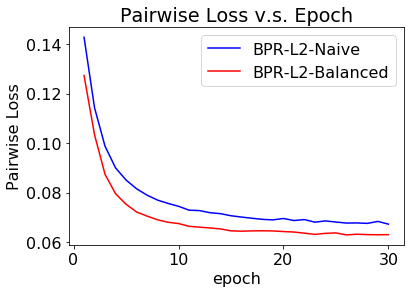
\includegraphics[width=.23\linewidth]{figures/ml-1mpairloss.png}}
%\subfloat[Hit Ratio(HR)@10]{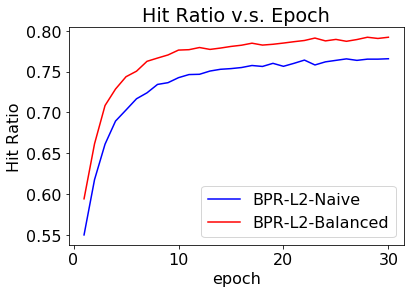
\includegraphics[width=.3\linewidth]{ml-1mhit.png}}
\subfloat[NDCG@10]{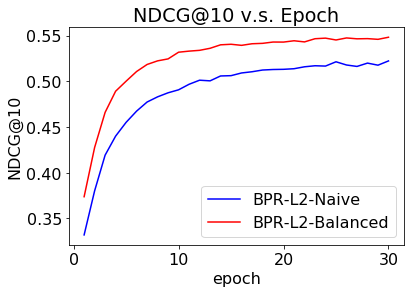
\includegraphics[width=.23\linewidth]{figures/ml-1mndcg.png}}
\subfloat[Pairwise Loss]{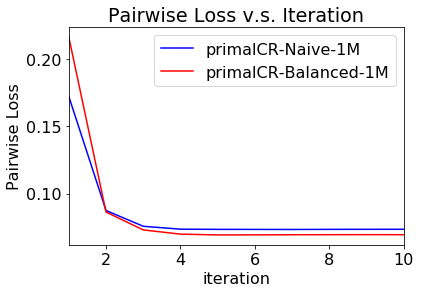
\includegraphics[width=.23\linewidth]{figures/primalCR_1M_pairloss.png}}
%\subfloat[Hit Ratio(HR)@10]{\includegraphics[width=.3\linewidth]{.png}}
\subfloat[NDCG@10]{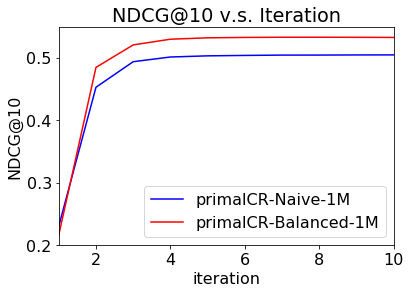
\includegraphics[width=.23\linewidth]{figures/primalCR_1M_ndcg.png}}
\caption{MovieLens1m, $r = 100$, $\lambda = 0.1$, stepsize $\eta = 0.01$, compare Naive Sampling and Balanced Sampling with BPR and PrimalCR(1 million subsampled pairs).}
\label{fig:1m_sample}

\vskip\baselineskip

\subfloat[Pairwise Loss]{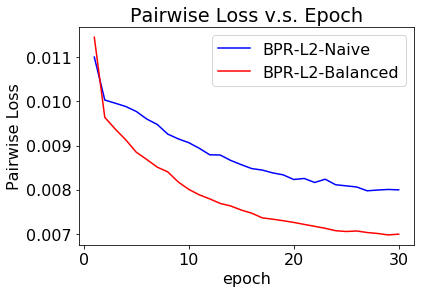
\includegraphics[width=.23\linewidth]{figures/ml-10mpairloss.png}}
%\subfloat[Hit Ratio(HR)@10]{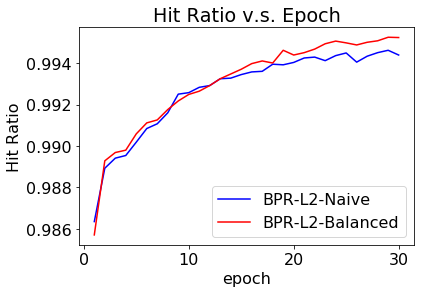
\includegraphics[width=.3\linewidth]{ml-10mhit.png}}
\subfloat[NDCG@10]{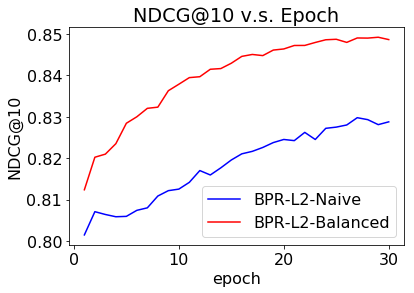
\includegraphics[width=.23\linewidth]{figures/ml-10mndcg.png}}
\subfloat[Pairwise Loss]{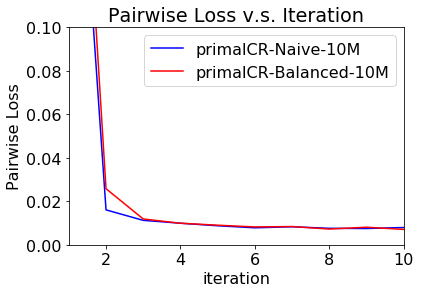
\includegraphics[width=.23\linewidth]{figures/primalCR_10M_pairloss.png}}
\subfloat[NDCG@10]{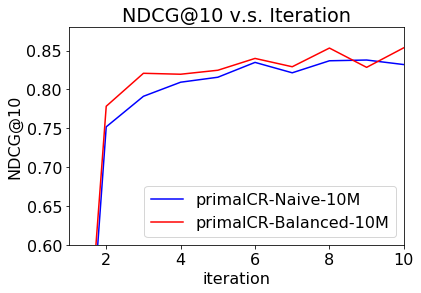
\includegraphics[width=.23\linewidth]{figures/primalCR_10M_ndcg.png}}
\caption{MovieLens10m, $r=100$, $\lambda = 0.1$, stepsize $\eta = 0.01$, compare Naive Sampling and Balanced Sampling with BPR and PrimalCR(10 million subsampled pairs)}
\label{fig:10m_sample}

\end{figure*}

\section{Experiments}
\label{sec:exp}

In this section, we compare the performance of balanced sampling strategy and naive uniform sampling strategy on real world datasets. {\color We also compare the efficient solvers using full data and subsampled data empirically}.

Studies \cite{cr}, \cite{crlinear} have argued that L2 hinge loss, $\mathcal{L}(x) = \max(0, 1- x)^2$, usually yields good performance in practice, so we adopt L2 hinge loss in our experiments. Similar experimental results can be drawn using other loss functions such as logistic loss. %Due to space limitation, we place the experimental result with logistic loss in the supplementary materials.

We include the following methods in our comparison:

\begin{itemize}
    \item \textsf{BPR-L2-Naive}: BPR with L2 hinge loss, constant stepsize and naive uniform sampling strategy using full data.
    \item \textsf{BPR-L2-Balanced}: BPR with L2 hinge loss, constant stepsize and our proposed balanced sampling strategy using full data.
    \item \textsf{PrimalCR-Naive}: PrimalCR with L2 hinge loss and subsampled pairs drawn from naive sampling strategy. 
    \item \textsf{PrimalCR-Balanced}: PrimalCR with L2 hinge loss and subsampled pairs drawn from balanced sampling strategy. We use the  available online Julia code with minor modifications. % {so that the input for the algorithm are pairs instead of a feedback matrix}.
    
    %Basically, \textsf{PrimalCR++} and \textsf{BPR-L2-Balanced} are optimizing the same problem, but \textsf{BPR-L2-Balanced} use full data for training and \textsf{PrimalCR++} use subsamples for training. We use the online available Julia code with minor modifications.
\end{itemize}
\laks{While all methods \textsf{PrimalCR-Balanced},  \textsf{PrimalCR-Naive}, and  \textsf{BPR-L2-Balanced}  optimize  the same objective function, \textsf{BPR} uses full data whereas \textsf{PrimalCR} uses subsampled data.} 

%Note that \textsf{PrimalCR-Balanced} and \textsf{PrimalCR-Naive} are optimizing the same problem as \textsf{BPR-L2-Balanced} and \textsf{BPR-L2-Naive} respectively, but \textsf{BPR-L2} uses full data for training and \textsf{PrimalCR} use subsampled data for training. 

% \begin{itemize}
%     \item Does balanced sampling strategy outperforms uniform sampling?
%     \item Can \textsf{primalCR++} with balanced negative sampling strategy beat \textsf{BPR} with full data on real world datasets?
%     %\item What is the trade-off between run time and ranking performance when we have more negative samples?
% \end{itemize}

\subsection{Data Statistics}

The statistics of data are shown in Table \ref{tab:data}

\begin{table}[t]
\small
\caption{Statistics of data}
\label{tab:data}
\vskip 0.15in
\begin{center}
\begin{small}
\begin{sc}
\begin{tabular}{lcccr}  \hline
Data set & \# users & \# items & \# ratings \\ \hline
MovieLens1M   & 6,040 & 3,952 & 1,000,209 \\
MovieLens10M  & 71,567 & 65,134 & 10,000,054 \\ \hline
\end{tabular}
\end{sc}
\end{small}
\end{center}
\end{table}

\laks{Note that MovieLens datasets are not naturally implicit feedback data, following the literature of recommendation systems with implicit feedback \cite{bpr, neural}, we treat all movies with rating as ``like", and all missing observations as   ``unrated". So our task now is predicting if a user is willing to rate an unrated movie.} 


\subsection{Evaluation Criterion}

To evaluate the performance of predictions, we adopt the popular leave-one-out evaluation which is widely used in the literature of recommender systems \cite{bpr, neural}. Namely we remove one positive feedback per user from our training set and put it into our test set, then we randomly select 100 negative feedbacks per user and put it into the test set. So we have 100 positive v.s. negative pairs for each user in our test set. We evaluate the ranking performance using the polular metrics  \textsf{Pairwise-Loss}, \textsf{Hit-Ratio(HR)@10}, and \textsf{NDCG@10}. 

We denote the test pairs as $\Omega_{test}$ and all the positive feedback in $\Omega_{test}$ as ${\Omega}_{test}^+$.

\begin{itemize}
    \item Pairwise-Loss: it represents the proportion of wrongly predicted triples.
    $$ \text{Pairwise-Loss} = \frac{1}{|\Omega_{test}|} \sum_{ (i,j,k) \in \Omega_{test} } 1(\hat{X}_{i,j} < \hat{X}_{i,k}) $$
    \item HR@$k$: it measures the proportion of users whose positive feedback (only one) is ranked among the  top $k$ in  the list. 
    $$ \text{HR@}k = \frac{1}{d_1}  \underset{R_{i,j} \in \Omega_{test}^+}{\sum} 1( \Pi_i(j) \leq k ) $$
    where $\Pi_i(j)$ is our ranking of item $j$ for user $i$.
    \item NDCG@$k$: as a popular criterion to evaluate ranking performance, it emphasizes more on the top-most rankings. It is defined as:
    $$ \text{NDCG@}k = \frac{1}{d_1} \sum_{i=1}^{d_1} \frac{\text{DCG@}k(i, \pi_{i})}{\text{DCG@}k(i, \pi^*_i)} $$
    where $\displaystyle \text{DCG@}k(i,\pi_i) = \sum_{j=1}^k \frac{2^{M_{i,\pi_i(j)}} - 1}{\log_2(j+1)}$, { $\pi_i(j)$ is the index of the $j$-th ranked item for user $i$ based on our prediction $\hat{X}$. DCG measures how well the top $k$ items are ranked.} 
\end{itemize}

\subsection{Implementation Details}

All of our code are implemented in Julia and all experiments are conducted on a server with 32 Intel Xeon  E5-2690 @ 2.90GHz CPUs and 64G memory. We use Julia v0.6.0 to run all the experiments. To tune the best parameters for each model, we further split a validation set from the training data by the same scheme of getting test data. 

\begin{figure*}[t!]
\centering
\subfloat[Pairwise Loss]{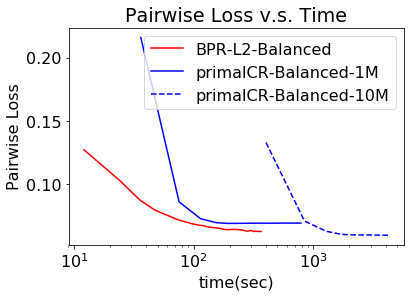
\includegraphics[width=.33\linewidth]{figures/CRBPRml-1mpairloss.png}}
\subfloat[Hit Ratio(HR)@10]{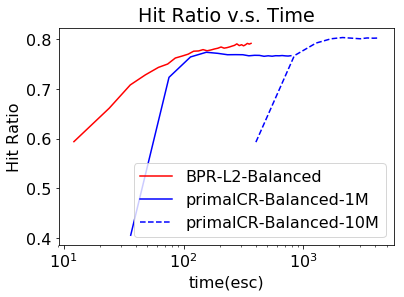
\includegraphics[width=.33\linewidth]{figures/CRBPRml-1mhit.png}}
\subfloat[NDCG@10]{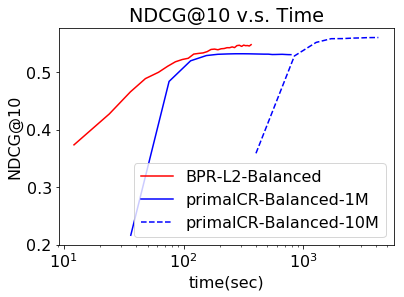
\includegraphics[width=.33\linewidth]{figures/CRBPRml-1mndcg.png}}
\caption{MovieLens1m, compare BPR-L2-balanced with full data and primalCR with 1 million and 10 million subsampled pairs drawn from balanced sampling, $r=100, \lambda = 0.1$}
\label{fig:CRBPRml-1m}

\vskip\baselineskip

\subfloat[Pairwise Loss]{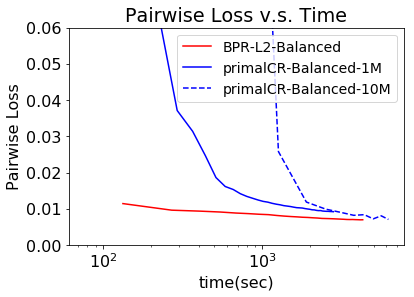
\includegraphics[width=.33\linewidth]{figures/CRBPRml-10mpairloss.png}}
\subfloat[Hit Ratio(HR)@10]{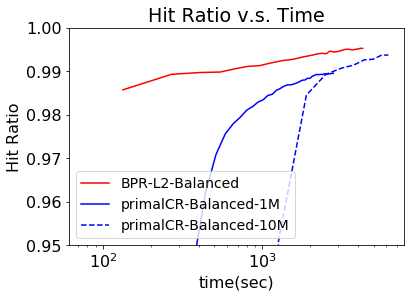
\includegraphics[width=.33\linewidth]{figures/CRBPRml-10mhit.png}}
\subfloat[NDCG@10]{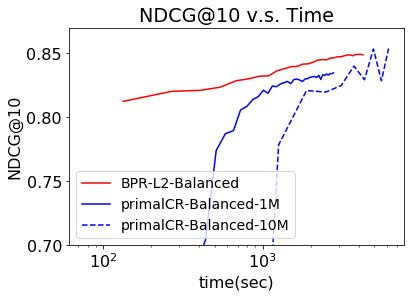
\includegraphics[width=.33\linewidth]{figures/CRBPRml-10mndcg.png}}
\caption{MovieLens10m, compare BPR-L2-balanced with full data and primalCR with 1 million and 10 million subsampled pairs drawn from balanced sampling, $r=100, \lambda = 0.1$}
\label{fig:CRBPRml-10m}


\end{figure*}


\subsection{Compare Sampling Strategies}

We compare the performance of balanced sampling and uniform sampling under the same parameters with different solvers. 
%The estimation of parameters for balanced sampling strategy is described in section \ref{sec:estimate}, so no more hyper-parameters are needed to tune for balanced sampling strategy.

For \textsf{BPR}, similar as \cite{bpr}, we set the number of data passed in one epoch equal to the total number of positive feedback, which is far less than the number of whole data $|\Omega|$.

For \textsf{PrimalCR}, we sample 1 million pairs for MovieLens1M and 10 million pairs for MovieLens10M.

As shown in Figures~\ref{fig:1m_sample}, \ref{fig:10m_sample}, balanced sampling outperforms uniform sampling in terms of Pairwise Loss, Hit Ratio and NDCG under both solvers, which is consistent with our theoretical analysis in Section \ref{sec:analysis}. We also observe that BPR works very well with MovieLens10m: Pairwise Loss is close to 0 and Hit Ratio is close to 100\%, which again demonstrates the effectiveness of pairwise model for ranking prediction.

% \subsection{Campare Sampling Strategies}

% We include the following sampling strategies into comparison:

% \begin{itemize}
%     \item Balanced Negative Sampling: our proposed negative sampling strategy in section \ref{sec:analysis}.
%     \item Naive Negative Sampling: the baseline, selecting $m$ negative samples uniform randomly from all possible negative feedbacks, mathematically saying $\cup_{i=1}^{d_1} \Omega_i^-$.
% \end{itemize}

\subsection{Compare \textsf{BPR} and \textsf{PrimalCR}}

%We randomly sample some negative feedbacks $\Omega^-$ so that the expected number of pairs of each user obey balanced sampling. The \textsf{pos/neg} ratio refers to the positive and negative feedbacks ratio $r = |\Omega^+|/|\Omega^-|$. The space complexity for \textsf{PrimalCR++} is $O(k(d_1+d_2) + (r+1)|\Omega^+| )$. To make \textsf{PrimalCR++} and \textsf{BPR} comparable in memory consumption, we try $r=1,2,3,4$ in the experiments.

%We use algorithm \ref{alg:sample_primalcr} to sample negative feedback for \textsf{PrimalCR++}. Under this sampling strategy, \textsf{PrimalCR++} and \textsf{BPR-L2-Balanced} are actually optimizing the same problem, where \textsf{PrimalCR++} use subsamples and \textsf{BPR-L2-Balanced} are using full data. $r$ refers to the ratio of the number of sampled negative feedback and the number of positive feedback, we show the result of $r=1$ and $4$ in this section.

We test \textsf{PrimalCR-Balanced} with 1 million subsampled pairs and 10 million subsampled pairs, and denote the results as \textsf{PrimalCR-Balanced-1M} and \textsf{PrimalCR-Balanced-10M} respectively.

As shown in Figures~\ref{fig:CRBPRml-1m}, \ref{fig:CRBPRml-10m}, for both MovieLens1m and MovieLens10m, \textsf{BPR-Balanced}, \textsf{PrimalCR-Balanced-1M} and \textsf{PrimalCR-Balanced-10M} can achieve the same level of Pairwise Loss, Hit Ratio and NDCG, which supports our {analysis about sample complexity} in Section \ref{sec:analysis} that using subsampled data is sufficient to achieve high prediction accuracy. In terms of convergence behavior, \textsf{BPR-Balanced} and \textsf{PrimalCR-Balanced-1M} perform similarly  on MovieLens1m, while \textsf{PrimalCR-Balanced-1M} is a little bit more stable since it uses true gradient unlike   SGD, which use noisy gradient. For large dataset like MovieLens10m, \textsf{BPR} converges faster than \textsf{PrimalCR} significantly. With huge-scale datasets, it is usually too expensive to solve them precisely and a moderate precision is enough to achieve good performance, which makes SGD especially suitable for these datasets.

To summarize, for large-scale datasets, \textsf{BPR} using full data based on SGD with balanced sampling is superior. For data with moderate size, we recommend using \textsf{PrimalCR} with subsamples drawn from balanced sampling { since we can achieve the same level of accuracy as BPR without spending time on tunning the stepsize}.







\section{Conclusion}
\label{sec:conclusion}

In this paper, we studied the theoretical properties of pair-wise collaborative ranking  over implicit feedback data, focusing on the sample complexity and generalization error bound. Our analysis shows that we are able to approximate the optimal noisy true error as long as our sample complexity is $\Omega \big( r(d_1+d_2)\ln^2(d_1d_2) \big)$. By manipulating the loss function or the subsampling strategy cleverly, we are able to approximate the optimal true error theoretically. 
%With our analytical result, we argue that pair-wise approaches could overcome the 2 challenges described in section \ref{sec:intro}, %namely the noisy observation and huge number of available pairs. 
In our experiments, we validate our theoretical analysis with real-world data. We also compare the state-of-the-art solvers for full data and subsampled data, and conclude that \textsf{BPR}, based on SGD, is more efficient for large-scale data while \textsf{PrimalCR}, with subsampled data using balanced sampling,  has a better convergence behavior on smaller data.  




% citation

\bibliographystyle{unsrt}
\bibliography{ref}

% \nocite{hsieh2015pu}
% \nocite{crlinear}
% \nocite{pcfpr}
% \nocite{cr}
% \nocite{bpr}
% \nocite{cfimplicit}
% \nocite{listwise}
% %\nocite{dr}
% %\nocite{facenet}
% \nocite{1bit}
% \nocite{uml}
% \nocite{maxmargin}
% \nocite{Mc}
% \nocite{neural}
% %\nocite{yang2014modeling}
% \nocite{negsample}
% \nocite{netflix}
% \nocite{yahoo!}
% \nocite{listcollaborativefiltering}
% \nocite{bprsample}
% \nocite{bprsample2}
% \nocite{collaborativeranking}
% \nocite{korenmf}
% \nocite{pmf}
% \nocite{sideinformation}
% %\nocite{bmc}
% %\nocite{millionsongs}


\section{Appendix}

\subsection{The relationship between $Y_{ijk}$ and $A_{ijk}$}
Given $Y_{ijk} = (1,1)$
\begin{equation}
\begin{aligned}
    & Pr[A_{ijk} = (1,1) ~|~ Y_{ijk} = (1,1)] = p_i^2 \\ 
    & Pr[A_{ijk} = (1,0) ~|~ Y_{ijk} = (1,1)] = p_i(1-p_i) \\
    & Pr[A_{ijk} = (0,1) ~|~ Y_{ijk} = (1,1)] = p_i(1-p_i) \\
    & Pr[A_{ijk} = (0,0) ~|~ Y_{ijk} = (1,1)] = (1-p_i)^2 \nonumber
\end{aligned}
\end{equation}
Given $Y_{ijk} = (1,0)$
\begin{equation}
\begin{aligned}
    & Pr[A_{ijk} = (1,0) ~|~ Y_{ijk} = (1,0)] = p_i \\ 
    & Pr[A_{ijk} = (0,0) ~|~ Y_{ijk} = (1,0)] = 1-p_i \\
 \nonumber
\end{aligned}
\end{equation}
Given $Y_{ijk} = (0,1)$
\begin{equation}
\begin{aligned}
    & Pr[A_{ijk} = (0,1) ~|~ Y_{ijk} = (0,1)] = p_i \\ 
    & Pr[A_{ijk} = (0,0) ~|~ Y_{ijk} = (0,1)] = 1-p_i \\
 \nonumber
\end{aligned}
\end{equation}
Given $Y_{ijk} = (0,0)$
\begin{equation}
\begin{aligned}
    & Pr[A_{ijk} = (0,0) ~|~ Y_{ijk} = (0,0)] = 1 \\ 
 \nonumber
\end{aligned}
\end{equation}

\subsection{Proof of Theorem 1}


Let $\displaystyle L(X) := \frac{1}{|\Omega_S|} \sum_{(i,j,k) \in \Omega_S}  \mathcal{L}( (R_{i,j} - R_{i,k})(X_{i,j} - X_{i,k}) )$
% $\Xi$ as all possible subsets $\{ \Omega ~|~ |\Omega| = m \}$

First, it is easy to see that under uniform sampling, we have $\mathbb{E}[L(X)] = R_A(X)$. 

Then we need to bound $\sup_{X \in \mathcal{X} } |L(X) - R_A(X)| $.

\begin{lemma}
\label{lemma:bound}
    With probability at least $1 - \delta/2$, 
    \begin{equation}
    \begin{aligned}
        \supX |L(X) - R_A(X)| \leq & 2 \alpha \sqrt{\frac{2\ln(2/\delta)}{m}} + 2\alpha \sqrt{ \frac{2\ln(4/\delta) }{d_1 d_2} } \\
        & + 2 C \sqrt{\frac{(d_1 + d_2)}{m}} \ln(d_1 d_2)
    \end{aligned}
    \end{equation}
\end{lemma}

\emph{Proof:}
Break the objective into 2 parts: 
%\begin{equation}
    \begin{align}
        \supX \Big|L(X) - R_A(X)\Big| \leq \supX \Big|L(X) - \mathbb{E}_{\Omega_S} [L(X) | R] \Big| \label{eq:part1}  \\ 
        + \supX \Big|\mathbb{E}_{\Omega_S} [L(X) | R] - R_A(X) \Big| \label{eq:part2}
    \end{align}
%\end{equation}

For the first part Eq \ref{eq:part1}, it can be easily bounded by \laks{the law of large numbers, and by using Hoeffding's inequality}.

Since $\mathcal{L}$ is 1-Lipschitz and $\underset{i,j}{\max} |X_{i,j}| \leq \alpha$, we have 
\[\Big|\mathcal{L}((R_{i,j} - R_{i,k})(X_{i,j} - X_{i,k})) - \mathcal{L}(0) \Big| \leq 2\alpha \] 
for $\forall 1 \leq i \leq d_1, 1 \leq j \leq d_2,  X \in \mathcal{X}$.

By Applying Hoeffding's Inequality, we know that

\begin{align}
    Pr\Big\{ \big|L(X) - \E_{\Omega_S}[ L(X) | R ]  \big| \geq \epsilon \Big\} \leq 2 \exp\Big\{-\frac{2m \epsilon^2}{(4\alpha)^2} \Big\} \nonumber
\end{align}

Let $2 \exp\left\{-\frac{2m \epsilon^2}{(4\alpha)^2} \right\} = \delta/4$, then with probability at least $1 - \delta/4$,

\begin{equation}
    \begin{aligned}
        \supX |L(X) - \mathbb{E}_{\Omega_S} [L(X) | R] | \leq 2 \alpha \sqrt{\frac{2\ln(8/\delta)}{m}}
        \label{eq:res_part1}
    \end{aligned}
\end{equation}

For the second part Eq \ref{eq:part2}, $\supX \big|\mathbb{E}_{\Omega_S} [L(X) | R] - R_A(X) \big|$ is a function of $R$, since $R_{i,j} \in \{0, 1\}$ are independent from each other, we can apply McDiarmid's Inequality \cite{Mc}.

First, it is easy to show that under uniform sampling, the expected number of pairs related with $R_{i,j}$ is $\frac{2m}{d_1 d_2}$, \laks{thus a single change of $R_{i,j}$ would  change $\E_{\Omega_S}[L(X)|R] $ by at most $c_{ij} = \frac{1}{m} \frac{2m}{d_1 d_2} 2\alpha = \frac{4 \alpha }{d_1 d_2} $.} 

By McDiarmid's inequality, with probability at least $1 - \delta/4$,

\begin{equation}
    \begin{aligned}
    & \sup_{X \in \mathcal{X}} \big| \mathbb{E}_{\Omega_S} [L(X) | R] - R_A(X) \big| \\
    \leq & \mathbb{E}_R \Big[ \sup_{X \in \mathcal{X}} \big|\mathbb{E}_{\Omega_S} [L(X) | R] - R_A(X) \big| \Big] + \sqrt{ \frac{\ln(4/\delta) \sum c_{ij}^2 }{2} } \nonumber
    \end{aligned}
\end{equation}

$\sum c_{ij}^2 = d_1 d_2 (\frac{4\alpha}{d_1 d_2})^2 = \frac{16 \alpha^2}{d_1 d_2}$. Plug it into the above formula, with probability at least $1 - \delta/4$

\begin{equation}
    \begin{aligned}
    & \sup_{X \in \mathcal{X}} \big| \mathbb{E}_{\Omega_S} [L(X) | R] - R_A(X) \big| \\
    \leq & \mathbb{E}_R \Big[ \sup_{X \in \mathcal{X}} \big|\mathbb{E}_{\Omega_S} [L(X) | R] - R_A(X) \big| \Big]  + 2\alpha \sqrt{ \frac{2\ln(4/\delta) }{d_1 d_2} }  \label{eq:res_part2}
    \end{aligned}
\end{equation}

Then all we need to do is to bound the term $\mathbb{E}_R \Big[ \sup_{X \in \mathcal{X}} \big|\mathbb{E}_{\Omega_S} [L(X) | A] - R_A(X) \big| \Big]$.

Introduce ``ghost variables" to construct Rademacher complexity \cite{uml}.

\begin{subequations}
\begin{align}
    & \mathbb{E}_R \Big[ \sup_{X \in \mathcal{X}} \big|\mathbb{E}_{\Omega_S} [L(X) | R] - R_A(X) \big| \Big] \\
    & \leq \E_R  \Big[ \sup_{X \in \mathcal{X}} \big|\mathbb{E}_{\Omega_S} [L(X) | R] - \E_{\Omega_S', R'} [L'(X) | R] \big| \Big] \nonumber \\
    & = \E_R \Big[ \supX \big| \E_{\Omega_S, \Omega_S', R'} \big[ \frac{1}{m}( \sum l_{ijk}(R) - \sum l_{i'j'k'}(R') ) \big] \big| \Big] \nonumber \\
    & \leq \frac{1}{m} \E_{\Omega_S, \Omega_S', R, R'} \Big[ \supX \big| \sum_{ \Omega_S} l_{ijk}(R) - \sum_{ \Omega_S'} l_{i'j'k'}(R')  \big| \Big] \nonumber \\
    & = \frac{1}{m} \E_{.., \sigma} \Big[ \supX \big| \sum \sigma_{ijk} \big( l_{ijk}(R) - l_{i'j'k'}(R') \big) \big| \Big] \nonumber \\
    & \leq \frac{2}{m} \E_{\Omega_S, R, \sigma} \Big[ \supX \big| \sum_{\Omega_S} \sigma_{ijk} \big( l_{ijk}(R) - l(0) \big)  \big| \Big]  \label{eq:rade} 
\end{align}
\end{subequations}

where $l_{ijk}(R)$ is a shortcut for $\mathcal{L}((R_{i,j} - R_{i,k})(X_{i,j} - X_{i,k}))$, $\sigma_{ijk}$s are random variables with equal chance to be $+1$ or $-1$. 

So far we have constructed the Rademacher complexity. then we need to derive a bound for it.

Since $\mathcal{L}$ is 1-Lipschitz,

\begin{subequations}
\begin{align}
    \ref{eq:rade} & \leq \frac{2}{m} \E \Big[ \supX \big| \sum_{\Omega_S} \sigma_{ijk} (R_{i,j} - R_{i,k})(X_{i,j} - X_{i,k}) \big| \Big] \label{eq:lip}
\end{align}
\end{subequations}

Define $\tilde{R}_{i,j} = R_{i,j} - \frac{1}{2}$, that is $\tilde{R}_{i,j} = \frac{1}{2}$ if $R_{i,j} = 1$ and $\tilde{R}_{i,j} = -\frac{1}{2}$ if $R_{i,j} = -1$.

Then

\begin{subequations}
\begin{align}
    \ref{eq:lip} & \leq \frac{2}{m} \E \Big[ \supX \big| \sum_{\Omega_S} \sigma_{ijk} (\tilde{R}_{i,j} - \tilde{R}_{i,k})(X_{i,j} - X_{i,k}) \big| \Big] \nonumber \\ 
    & \leq \frac{2}{m}\bigg\{ \E \Big[ \supX \big| \sum_{\Omega_S} \sigma_{ijk} \tilde{R}_{i,j}(X_{i,j} - X_{i,k}) \big| \Big] \Big \nonumber \\   
    &~~~~ + \E \Big[ \supX \big| \sum_{\Omega_S} \sigma_{ijk} \tilde{R}_{i,k}(X_{i,j} - X_{i,k}) \big| \Big] \bigg\} \nonumber \\
    & = \frac{2}{m}\bigg\{ \E \Big[ \supX \big| \sum_{\Omega_S} \frac{1}{2}\sigma_{ijk} (X_{i,j} - X_{i,k}) \big| \Big] \Big \nonumber \\   
    &~~~~ + \E \Big[ \supX \big| \sum_{\Omega_S} \frac{1}{2} \sigma_{ijk} (X_{i,j} - X_{i,k}) \big| \Big] \bigg\}  \label{eq:transform} \\
    & = \frac{2}{m} \E \Big[ \supX \big| \sum_{\Omega_S} \sigma_{ijk} (X_{i,j} - X_{i,k}) \big| \Big] \label{eq:res1}
\end{align}
\end{subequations}

Eq \ref{eq:transform} is true since $\frac{1}{2} \sigma_{ijk}$ has the same distribution as $\sigma_{ijk} \tilde{R}_{i,j}$.

\begin{align}
    & \supX \big| \sum_{\Omega_S} \sigma_{ijk} (X_{i,j} - X_{i,k}) \big| \label{eq:sparse} \\
    = & \supX \big| \sum_{i,j,k} \sigma_{ijk} \xi_{ijk}(X_{i,j} - X_{i,k}) \nonumber \big|
\end{align}

where $\xi_{ijk}$ is a random variable that represents the number of time that $(i,j,k)$ is sampled(highly sparse).

Follow the same framework of \cite{cr}, let $M$ be the matrix s.t. $M_{i,j} = \sum_k (\sigma_{ijk} \xi_{ijk} - \sigma_{ikj}\xi_{ikj})$.

\begin{align}
    \ref{eq:sparse} = \supX \text{tr}(M^TX) = \sqrt{\lambda d_1 d_2} \|M\|
\end{align}
where $\| \cdot \|$ is the operator norm.

Use Lemma A.1 from \cite{cr}. 

$$\E \big[ \|M\| \big] \leq C\sqrt{\frac{m(d_1 + d_2)}{d_1 d_2}} \log(d_1 d_2)$$

Plug it into Eq \ref{eq:res1}, we get 

\begin{equation}
    \begin{aligned}
    & \mathbb{E}_R \Big[ \sup_{X \in \mathcal{X}} \big|\mathbb{E}_{\Omega_S} [L(X) | R] - R_A(X) \big| \Big] \nonumber \\
    \leq & ~ 2 C \sqrt{\frac{\lambda (d_1 + d_2)}{m}} \ln(d_1 d_2) \label{eq:res_part3}
    \end{aligned}
\end{equation}

Put Eq \ref{eq:res_part1}, \ref{eq:res_part2}, \ref{eq:res_part3} together. With probability at least $1 - \delta /2$,

\begin{equation}
    \begin{aligned}
        \supX |L(X) - R_A(X)| \leq & 2 \alpha \sqrt{\frac{2\ln(8/\delta)}{m}} + 2\alpha \sqrt{ \frac{2\ln(4/\delta) }{d_1 d_2} } \\
        & + 2 C \sqrt{\frac{\lambda (d_1 + d_2)}{m}} \ln(d_1 d_2)
    \end{aligned}
\end{equation}

This completes the proof of Lemma \ref{lemma:bound}.
\qed 

We now return to Theorem 1 % \ref{thm:noisy}.

For $\forall \tilde{X} \in \mathcal{X}$, with probability $1 - \delta$,
\begin{equation}
    \begin{aligned}
        R_A(\hat{X}) & \leq L(\hat{X}) + T &~~~\text{(lemma \ref{lemma:bound})} \\
        & \leq L(\tide{X}) + T &\text{(Definition of $\hat{X}$)} \\
        & \leq R_A(\tilde{X}) + 2T  &\text{(lemma \ref{lemma:bound})} \nonumber    
    \end{aligned}
\end{equation}

where
\begin{align}
    T = &~ 2 \alpha \sqrt{\frac{2\ln(8/\delta)}{m}} + 2\alpha \sqrt{ \frac{2\ln(4/\delta) }{d_1 d_2} } \nonumber \\
     & + 2 C \sqrt{\frac{\lambda(d_1 + d_2)}{m}} \ln(d_1 d_2) \nonumber
\end{align}


This completes the proof of Theorem 1. \qed 

%\ref{thm:noisy}.



%\section*{Proof of theorem \ref{thm:truerisk}}
\subsection*{Proof of Theorem 2}

Build an auxiliary loss function for $\tilde{\mathcal{L}}$.
\begin{equation}
    \begin{aligned}
        & \tilde{\mathcal{L}}_A(A_{ijk}, X_{i,j}, X_{i,k}, p_i) =  \\
        &\begin{cases}
             \mathcal{L}(0) & \text{if}~ A_{ijk} = (0,0) \\
             \frac{ \mathcal{L}(X_{i,j} - X_{i,k}) - (1-p_i) \mathcal{L}(0)  }{p_i} &  \text{if}~ A_{ijk} = (1,0) \\
             \frac{ \mathcal{L}(X_{i,k} - X_{i,j}) - (1-p_i) \mathcal{L}(0) }{p_i} &  \text{if}~ A_{ijk} = (0,1) \\
             \frac{ -(1-p_i)[\mathcal{L}(X_{i,j} - X_{i,k}) + \mathcal{L}(X_{i,k} - X_{i,j})  ] }{p_i^2}
             + & \frac{p_i^2 - 2p_i + 2}{p_i^2} \mathcal{L}(0) \\  & \text{if}~ A_{ijk} = (1,1)
        \end{cases}
    \end{aligned}
    \label{eq:modifiedloss}
\end{equation}
Denote 
$$\tilde{L}_A(X) := \frac{1}{|\Omega_S|} \sum_{(i,j,k) \in \Omega_S}  \tilde{\mathcal{L}}_A( (R_{i,j} - R_{i,k})(X_{i,j} - X_{i,k}) )$$

\begin{lemma}
For $\forall X \in \R^{d_1 \times d_2}$, $\mathbb{E}[\tilde{L}_A(X)] = R_Y(X) $
\label{lemma:exp}
\end{lemma}

\red{The proof of Lemma \ref{lemma:exp} is straight forward by expanding $\mathbb{E}[\tilde{L}_A(X)]$, and we skip it due to space limitation. } \qed

% \emph{Proof:}
% \begin{equation}
%     \begin{aligned}
%         &\mathbb{E}[\tilde{L}_A(X)]  =  \frac{1}{|\Omega_S|} \sum_{(i,j,k) \in \Omega_S} \mathbb{E}\Big[ \mathcal{L}( (R_{i,j} - R_{i,k})(X_{i,j} - X_{i,k}) ) \Big] \\
%          = & \frac{1}{d_1 d_2(d_2-1)} \sum_{i=1}^{d_1} \sum_{\substack{j,k=1\\ j \neq k} }^{d_2} \Big[ Pr[Y_{ijk} = (0,0)] \tilde{\mathcal{L}}_A((0,0))  \\
%          & + Pr[Y_{ijk} = (1,0)]\big( p_i \tilde{\mathcal{L}}_A\big((1,0) \big) + (1-p_i) \tilde{\mathcal{L}}_A\big((0,0) \big) \big) \\
%          & + Pr[Y_{ijk} = (0,1)]\big( p_i \tilde{\mathcal{L}}_A\big((0,1) \big) + (1-p_i) \tilde{\mathcal{L}}_A\big((0,0) \big) \big) \\
%          & + Pr[Y_{ijk} = (1,1)]\big( p_i^2 \tilde{\mathcal{L}}_A\big((1,1) \big) + (1-p_i)^2 \tilde{\mathcal{L}}_A\big((0,0) \big) \\
%          & + p_i(1-p_i)[\tilde{\mathcal{L}}_A\big((1,0)\big) + \tilde{\mathcal{L}}_A\big((0,1)\big)]  \big)   \Big] \\
%          = & \frac{1}{d_1 d_2(d_2-1)} \sum_{i=1}^{d_1} \sum_{\substack{j,k=1\\ j \neq k} }^{d_2} \Big[ Pr[Y_{ijk} = (0,0)] \mathcal{L}(0) \\
%          & \qquad \qquad \quad + Pr[Y_{ijk} = (1,0)] \mathcal{L}(X_{i,j} - X_{i,k}) \\
%          & \qquad \qquad \quad + Pr[Y_{ijk} = (0,1)] \mathcal{L}(X_{i,k} - X_{i,j}) \\
%          & \qquad \qquad \quad + Pr[Y_{ijk} = (1,1)] \mathcal{L}(0) \Big] \\
%          = & R_Y(X)
%     \end{aligned}
% \end{equation}

% where $ \tilde{\mathcal{L}}_A\big((a,b) \big) $ is a shortcut for $\tilde{\mathcal{L}}_A\big( (a,b), X_{i,j}, X_{i,k}, p_i \big)$, $a,b \in \{0,1\}$ \qed

Back to the proof of Theorem 2. It is obvious to see that Eq 4.1 
%\ref{eq:noisy_erm} 
has the same solution under $\tilde{\mathcal{L}}$ and $\tilde{\mathcal{L}}_A$ since their difference is a constant term.

\laks{We can use an argument analogous to that in the proof of Theorem 1 here}, the only difference being w.r.t.  the maximum change of $\tilde{\mathcal{L}}_A$ and the Lipschitz constant of $\tilde{\mathcal{L}}_A$. 

It is easy to show that 
the maximum change of $\tilde{\mathcal{L}}_A$ is $\kappa_1 \leq 2 \underset{1\leq i \leq d_1}{\max} \bigg\{ \max \Big\{ \frac{4\alpha}{p_{i}}, \frac{4(1-p_i)\alpha}{p_i^2} \Big\} \bigg\}$
% \begin{align}
%     \kappa_1 := & \max_{X \in \mathcal{X}, A \in \mathcal{H}_A}{ \tilde{\mathcal{L}}_A(A_{ijk}, X_{i,j}, X_{i,k}) } \nonumber \\
%         & - \min_{X \in \mathcal{X}, A\in \mathcal{H}_A}{ \tilde{\mathcal{L}}_A(A_{ijk}, X_{i,j}, X_{i,k}) } \nonumber \\ 
%     \leq & 2 \max_{X \in \mathcal{X}, A\in \mathcal{H}_A} \big| \tilde{\mathcal{L}}_A(A_{ijk}, X_{i,j}, X_{i,k}) - \mathcal{L}(0) \big| \\
%     \leq & 2 \underset{1\leq i \leq d_1}{\max} \bigg\{ \max \Big\{ \frac{4\alpha}{p_{i}}, \frac{4(1-p_i)\alpha}{p_i^2} \Big\} \bigg\} \nonumber
%     %\frac{2\alpha}{p_i} + \frac{2(p_i-1)^2}{p_i^2} \mathcal{L}(0), \nonumber \\ & \frac{4-2p_i}{p_i^2} \alpha + \frac{2(p_i-1)^2}{p_i^2} \mathcal{L}(0) \Big\} \bigg\} \nonumber
% \end{align}
and the Lipschitz constant of $\tilde{\mathcal{L}}_A$ to the respect of $X_{i,j} - X_{i,k}$ is at most $\kappa_2 = \underset{1\leq i\leq d_1}{\max}\{ \max\{\frac{1}{p_i}, \frac{2(1 - p_i)}{p_i^2}\} \}$.

Plug $\kappa_1$ and $\kappa_2$ into the proof, we can get

With probability $1 - \delta/2$

\begin{equation}
    \begin{aligned}
    \sup_{X \in \mathcal{X} } |\tilde{L}_A(X) - R_Y(X)| & \leq \kappa_1 \sqrt{\frac{\ln(8/\delta)}{2m}} + \kappa_1 \sqrt{ \frac{2\ln(4/\delta) }{d_1 d_2} } \\
        & + 2 \kappa_2 C \sqrt{\frac{\lambda(d_1 + d_2)}{m}} \ln(d_1 d_2) \label{eq:helper_thm2}
    \end{aligned}
\end{equation}

\laks{similarly} to Theorem 1. %\ref{thm:noisy}

For $\forall \tilde{X} \in \mathcal{X}$, with probability $1 - \delta$,
\begin{equation}
    \begin{aligned}
        R_Y(\hat{X}) & \leq \tilde{L}_A(\hat{X}) + T &~~~\text{(according to Eq \ref{eq:helper_thm2})} \\
        & \leq \tilde{L}_A(\tide{X}) + T &\text{(Definition of $\hat{X}$)} \\
        & \leq R_Y(\tilde{X}) + 2T  &\text{(according to Eq \ref{eq:helper_thm2})} \nonumber    
    \end{aligned}
\end{equation}

where
\begin{align}
T = & \kappa_1 \sqrt{\frac{\log(8/\delta)}{2m}} + \kappa_1 \sqrt{ \frac{2\ln(4/\delta) }{d_1 d_2} } \nonumber \\
      & + 2 \kappa_2 C \sqrt{\frac{\lambda(d_1 + d_2)}{m}} \ln(d_1 d_2) \nonumber 
\end{align}
%$\kappa_1 =  2 \underset{1\leq i \leq d_1}{\max} \{ \max \{ \frac{4\alpha}{p_{i}}, \frac{4(1-p_i)\alpha}{p_i^2} \} \}$, 
%        $\kappa_2 = \underset{1\leq i\leq d_1}{\max}\{ \max\{\frac{1}{p_i}, \frac{2(1 - p_i)}{p_i^2}\} \}$

This completes the proof of Theorem 2. \qed  .%\ref{thm:truerisk}.


% if $\mathcal{L}$ is 1-Lipschitz, then it is easy to show that the Lipschitz constant for $\tilde{\mathcal{L}}$ and $\tilde{\mathcal{L}}_A$ is $\kappa = \underset{1 \leq 1 \leq d_1}{\max}\{ \max\{\frac{1}{p_i}, \frac{2}{1-p_i}\} \}$.



% For $\forall \tilde{X} \in \mathcal{X}$, with probability $1 - \delta$,
% \begin{equation}
%     \begin{aligned}
%         R_Y(\hat{X}) \leq \tilde{L}_A(\hat{X}) + T \leq \tilde{L}_A(\tide{X}) + T \leq R_Y(\tilde{X}) + 2T
%     \end{aligned}
% \end{equation}
% where $T = \kappa \frac{4\alpha}{\sqrt{m \delta}} + 4 \kappa \alpha \sqrt{ \frac{2 \ln(4/\delta) }{d_1d_2} } + 2 \kappa C \sqrt{\frac{\lambda(d_1 + d_2)}{m}} \log(d_1 d_2)$

%\section{Proof for Theorm \ref{thm:truerisk2}}
\subsection{Proof of Theorem 3 and Theorem 4}

Theorem 3 and Theorem 4 can be proved using an argument analogous to that for Theorem 2. Here we just present the sketch of our proof.

For Theorem 3, we use the following auxiliary loss function for $\tilde{\mathcal{L}}^*$.

\begin{equation}
    \begin{aligned}
        & \tilde{\mathcal{L}}^*_A(A_{ijk}, X_{i,j}, X_{i,k}, p_i) = & \\
        & \begin{cases}
             \mathcal{L}(0) & \text{if}~ A_{ijk} = (0,0) \\
             \frac{ \mathcal{L}(X_{i,j} - X_{i,k}) - (1-p_i) \mathcal{L}(0)  }{p_i} &  \text{if}~ A_{ijk} = (1,0) \\
             \frac{ \mathcal{L}(X_{i,k} - X_{i,j}) - (1-p_i) \mathcal{L}(0) }{p_i} &  \text{if}~ A_{ijk} = (0,1) \\
             \mathcal{L}(0) &  \text{if}~ A_{ijk} = (1,1)
        \end{cases}
    \end{aligned}
    \label{eq:modifiedloss}
\end{equation}

Denote 
$$\tilde{L}^*_A(X) := \frac{1}{|\Omega_S|} \sum_{(i,j,k) \in \Omega_S}  \tilde{\mathcal{L}}^*_A( (R_{i,j} - R_{i,k})(X_{i,j} - X_{i,k}) )$$

We break the objective into 3 parts, 

\begin{align}
    \supX  | \tilde{L}_A^*(X) & -  R_Y(X)|  \leq \supX | \tilde{L}_A^*(X) - \mathbb{E}_{\Omega_S} [\tilde{L}_A^*(X) | R] | \nonumber \\ 
    & + \supX |\mathbb{E}_{\Omega_S} [\tilde{L}_A^*(X) | R] - \mathbb{E}_{\Omega_S, R} [\tilde{L}_A^*(X)]| \nonumber \\
    & + \supX |\mathbb{E}_{\Omega_S, R} [\tilde{L}_A^*(X)] - R_Y(X) | \label{eq:constgap}
\end{align}

The first two parts can be bounded using the same arguments analogous to that for Theorem 1 and 2. It is also easy to show that $\ref{eq:constgap} \leq 4\alpha(1 - p_{min}) \E\left[ \bm{1}_{Y_{ijk} = (1,1)} \right]$.

For Theorem 4, we introduce the idea of balanced sampleing. Note that balanced sampling has the same expected true error as the weighted loss used in Theorem 3. Using the same argument as Theorem 3, it is easy to show that balanced sampling and weighted loss share the same property. \qed

% Build an auxiliary loss function for $\tilde{\mathcal{L}}^*$.

% \begin{equation}
%     \begin{aligned}
%         & \tilde{\mathcal{L}}^*_A(A_{ijk}, X_{i,j}, X_{i,k}, p_i) = & \\
%         & \begin{cases}
%              \mathcal{L}(0) & \text{if}~ A_{ijk} = (0,0) \\
%              \frac{ \mathcal{L}(X_{i,j} - X_{i,k}) - (1-p_i) \mathcal{L}(0)  }{p_i} &  \text{if}~ A_{ijk} = (1,0) \\
%              \frac{ \mathcal{L}(X_{i,k} - X_{i,j}) - (1-p_i) \mathcal{L}(0) }{p_i} &  \text{if}~ A_{ijk} = (0,1) \\
%              \mathcal{L}(0) &  \text{if}~ A_{ijk} = (1,1)
%         \end{cases}
%     \end{aligned}
%     \label{eq:modifiedloss}
% \end{equation}
% %where $t$ is going to be determined later.
% Denote 
% $$\tilde{L}^*_A(X) := \frac{1}{|\Omega_S|} \sum_{(i,j,k) \in \Omega_S}  \tilde{\mathcal{L}}^*_A( (R_{i,j} - R_{i,k})(X_{i,j} - X_{i,k}) )$$
% We also need to bound $\supX |L_A^*(X) - R_Y(X)|$, but differently from the proof of Theorem 1% \ref{thm:noisy}
% , now we need to break the objective into 3 parts.

% % \begin{align}
% %     \supX |L_A^*(X) - R_Y(X)| \leq \supX |L_A^*(X) - \mathbb{E}_{\Omega_S} [L_A^*(X) | R] | \nonumber \\ 
% %     + \supX |\mathbb{E}_{\Omega_S} [L_A^*(X) | R] - \mathbb{E}_{\Omega_S, R} [L_A^*(X)]| \nonumber \\
% %     + \supX |\mathbb{E}_{\Omega_S, R} [L_A^*(X)] - R_Y(X) | \label{eq:constgap}
% % \end{align}

% For the first two parts, the proof is the same as Theorem 1.
% %\ref{thm:noisy}. 
% The Lipschitz  constant of  of $\tilde{\mathcal{L}}_A^*$ is $1/p_{min}$. And $\max\{ \tilde{\mathcal{L}}_A \} - \min\{\tilde{\mathcal{L}}_A\} = \frac{4\alpha}{p_{min}}$, where $p_{min} = \min \{ p_i \}$.

% For the third part, it is the gap between two expectations. Plugging in  $L_A^*(X)$ into Eq \ref{eq:constgap}, 

% \begin{subequations}
% \begin{align}
%     \ref{eq:constgap} = & \supX \bigg| \E\Big[ \bm{1}_{Y_{ijk} = (1,1)} \Big( (p_i^2 + (1-p_i)^2) \mathcal{L}(0) \nonumber \\
%     & \qquad + (1-p_i)(\mathcal{L}(X_{i.j} - X_{i,k}) + \mathcal{L}(X_{i,k} - X_{i,j})) \nonumber \\
%     & \qquad + 2(1-p_i)^2 \mathcal{L}(0) - \mathcal{L}(0) \Big) \Big] \bigg| \nonumber \\
%     & =  \supX \bigg| \E\Big[ \bm{1}_{Y_{ijk} = (1,1)} (1-p_i)\big(\mathcal{L}(X_{i.j} - X_{i,k}) \nonumber \\
%     & \qquad \quad + \mathcal{L}(X_{i,k} - X_{i,j}) - 2 \mathcal{L}(0) \big) \Big] \bigg| \nonumber \\
%     & \leq 4\alpha(1 - p_{min}) \E\Big[ \bm{1}_{Y_{ijk} = (1,1)} \Big]   \label{eq:gapres}
% \end{align}
% \end{subequations}

% Eq \ref{eq:gapres} is true since $\mathcal{L}$ is 1-Lipschitz.

% So, with probability at least $1-\delta/2$

% \begin{equation}
%     \begin{aligned}
%     \sup_{X \in \mathcal{X} } |\tilde{L}_A^*(X) - R_Y(X)| & \leq  2 \alpha \kappa \sqrt{\frac{\log(8/\delta)}{2m}} + 2\alpha \kappa \sqrt{ \frac{2\ln(4/\delta) }{d_1 d_2} } \\
%         & + 2 \kappa C \sqrt{\frac{(d_1 + d_2)}{m}} \log(d_1 d_2) \\
%         & +   4\alpha(1 - p_{min}) \E\Big[ \bm{1}_{Y_{ijk} = (1,1)} \Big] \label{eq:thm3_helper}
%     \end{aligned}
% \end{equation}

% where $\kappa = \max\{1/p_i\}$.

% Similarly,
% for $\forall \tilde{X} \in \mathcal{X}$, with probability $1 - \delta$,
% \begin{equation}
%     \begin{aligned}
%         R_Y(\hat{X}) & \leq \tilde{L}_A(\hat{X}) + T &~~~\text{(According to Eq \ref{eq:thm3_helper})} \\
%         & \leq \tilde{L}_A(\tide{X}) + T &\text{(Definition of $\hat{X}$)} \\
%         & \leq R_Y(\tilde{X}) + 2T  &\text{(According to Eq \ref{eq:thm3_helper})} \nonumber    
%     \end{aligned}
% \end{equation}

% This completes the proof for Theorem 3. \qed 

% \subsection{Proof for Theorem 4}

% \laks{Theorem 4 can be proved using an argument analogous to that for Theorem 3. Specifically, 
%  we need to build an auxiliary function and bound the difference between the empirical risk and the true error. Note that balanced sampling has the same expected true error as the weighted loss used in Theorem 3. Using the same argument as Theorem 3, it is easy to show that balanced sampling and weighted loss share the same property. We omit the details.} 



\end{document}
